% 原书 p.141–p.147（PDF p.149–p.155）
\chapter{定量刻画（Quantitative Characterizations）}

% >>> p149
概括地说，辛几何主要研究以下三类对象：哈密顿动力学、拉格朗日子流形与刘维尔
（Liouville）区域。它们提供了考察辛刚性的各式平台。与数学中许多其他分支不同，
由于辛几何深植于哈密顿动力学（其根源最终可追溯到函数），定量研究不仅可能，而且
在辛几何中影响深远。这里，人们可以用刚性所能达到的程度来刻画刚性，而不是仅仅
给出「是（存在）」或「否（不存在）」这样简单的回答。这一点在 Gromov 非压缩定理
（定理 1.5.1）中体现得尤为清楚：辛嵌入存在的门槛，恰是若干区域某些尺寸之间的、
相对的定量比较。本章将引入多种概念，用以定量刻画哈密顿动力学与刘维尔区域。对
拉格朗日子流形的定量研究将推迟到第 9 章。在这些定量刻画之下，人们能够描述一个
哈密顿动力学「有多混沌」；也能够说出两个刘维尔区域之间一个精心设计的标量差异，
而后者同样是一个辛不变量。

\section{Hofer 几何（Hofer's Geometry）}

\begin{keytakeaways}
\begin{itemize}
  \item 几何图像：把 Hamilton 微分同胚群 $\Ham(M,\omega)$ 本身当作一个度量空间来
        研究——元素「有多大」由生成它的哈密顿函数的振幅（最大值减最小值）来度量，
        「是否混沌」于是成为一个度量几何问题。
  \item 核心工具：Hofer 范数 $\|\cdot\|_{\mathrm{Hofer}}$（式 (6.1)）与由它导出的
        双不变距离 $d_{\mathrm{Hofer}}$；前者只涉及 $C^0$ 量、不涉及 $H$ 的导数。
  \item 关键定理：Hofer 范数的非退化性（定理 6.1.1）是全部定量理论的基础；位移
        能量 $e(A)$（定义 6.1.2）是辛容量的雏形，内部非空的集合必有 $e(A)>0$
        （定理 6.1.2）。
  \item 本节结论：$\bigl(\Ham(M,\omega),d_{\mathrm{Hofer}}\bigr)$ 是真正的度量空间；
        位移能量是辛同胚不变量，且球 $B^{2n}(r)$ 的位移能量为 $\pi r^2$。
\end{itemize}
\end{keytakeaways}

Hofer 几何指的是：直接在辛流形 $(M,\omega)$ 的哈密顿微分同胚群 $\Ham(M,\omega)$ 上
研究哈密顿动力学的一种几何进路（见 1.7 节）。这与纯粹从微分方程出发研究动力学的
经典方法大相径庭。这里的「几何」意指：人们可以定量地度量 $\Ham(M,\omega)$ 中元素
的大小，从而把「是否混沌」转化为一个度量几何问题。整个故事可追溯到 Banyaga 的
下述基本结果。

\whead{事实}{6.1.1$^{[23]}$}给定辛流形 $(M,\omega)$，则其哈密顿微分同胚群
$\Ham(M,\omega)$ 中的任意一条道路都是哈密顿流（见图 6.1）。换言之，对任意道路
$\{\varphi_t\}_{t\in[0,1]}\subset\Ham(M,\omega)$，只要 $\varphi_0=\varphi$、
$\varphi_1=\psi$，就存在 $H\colon[0,1]\times M\to\R$，使得

% >>> p150
$d\varphi_t/dt=X_{H_t}(\varphi_t)$。

\begin{figure}[htbp]
  \centering
  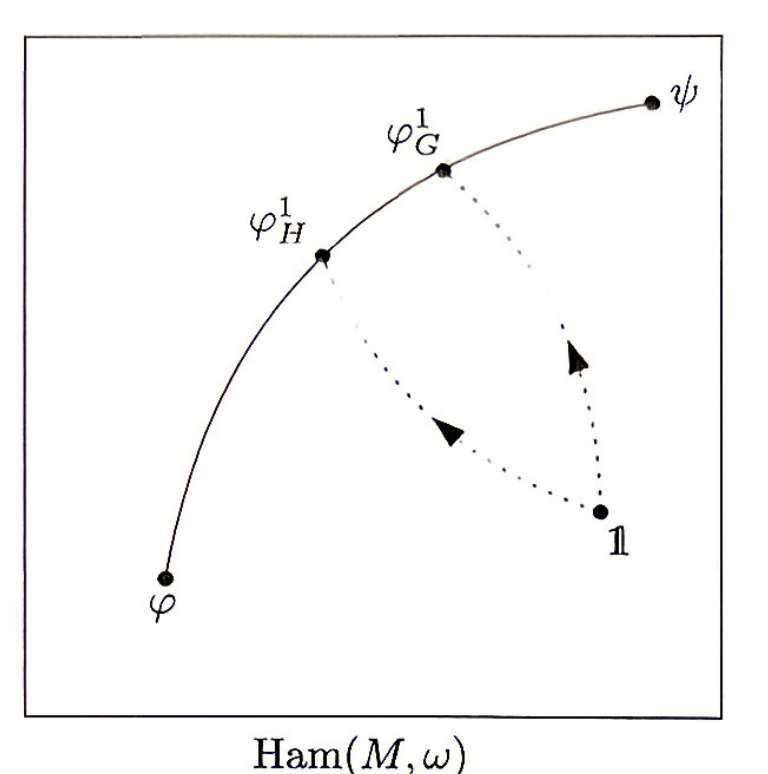
\includegraphics[width=0.46\linewidth]{figures/fig_p150_1.png}
  \caption*{图 6.1\quad 连接 $\varphi$ 与 $\psi$ 的道路上每一点都是某个时间 1 映射
    （原书 p.142, Figure 6.1；PDF p.150）}
\end{figure}

这是一个极为惊人的结果：道路 $\{\varphi_t\}_{t\in[0,1]}$ 上的每一点都是某个哈密顿
同痕的时间 1 映射，而上述事实 6.1.1 表明，(依赖于时间的) 哈密顿函数竟能通过单一的
哈密顿同痕把这一切「统一」起来。

另一方面，对任意哈密顿函数 $H\colon[0,1]\times M\to\R$，考虑下述量：

\begin{equation}\tag{6.1}
  \|H\|_{\mathrm{Hofer}}
  :=\int_0^1\left(\max_M H_t-\min_M H_t\right)dt.
\end{equation}

注意 $\|\cdot\|_{\mathrm{Hofer}}$ 是 $C^0$ 意义下的（不涉及 $H$ 的任何导数），并且
在平移 $H\to H+c$（$c$ 为任意常数）下不变。可以作如下规范化：若 $M$ 是闭的，则称
$H$ 是\textbf{规范化}的，如果 $H_t$ 的均值满足下述方程

\[
  \int_0^1\int_M H_t\,\mathrm{dvol}\,dt=0.
\]

若 $M$ 是开的（非紧的，或者紧但边界非空），则称 $H$ 是\textbf{规范化}的，如果对
每个 $t\in[0,1]$，函数 $H_t$ 在 $M$ 中具有紧支撑。

现在把事实 6.1.1 与 $\|\cdot\|_{\mathrm{Hofer}}$ 结合起来，便得到本节的核心定义。

\begin{wdefn}{6.1.1（Hofer 范数）}
  设 $(M,\omega)$ 是辛流形，$\Ham(M,\omega)$ 为其哈密顿微分同胚群。则对任意
  $\varphi\in\Ham(M,\omega)$，定义 $\varphi$ 的\textbf{Hofer 范数}为
  \[
    \|\varphi\|_{\mathrm{Hofer}}
    :=\inf\left\{\|H\|_{\mathrm{Hofer}}\;\middle|\;
    \begin{array}{l}
      H\ \text{是生成一条连接}\ \mathbf{1}\ \text{与}\ \varphi\ \text{的道路}\\
      \{\varphi_t\}_{t\in[0,1]}\ \text{的哈密顿函数}
    \end{array}\right\}.
  \]
\end{wdefn}

% [Tutor Note: 易错预警——定义 6.1.1 中的下确界取了「两重」：既对一切连接
% $\mathbf{1}$ 与 $\varphi$ 的道路 $\{\varphi_t\}$ 取，也对生成每条固定道路的一切
% 哈密顿函数 $H$ 取。由事实 6.1.1，一条道路总可由某个 $H$ 生成；而生成同一道路的
% 两个 $H$ 只相差一个依赖于时间的常数 $c(t)$（因为 $X_{H_t}$ 只取决于 $H_t$ 的
% 微分），故 (6.1) 的振幅 $\max H_t-\min H_t$ 在 $H\mapsto H+c(t)$ 下不变，从而
% 规范化与否不影响范数值。建议核对：$H_t$ 的常数项确实不进入 $\|H\|_{\mathrm{Hofer}}$。]

% [Tutor Note: 含糊点拨——事实 6.1.1 是 Banyaga 定理（$\Ham(M,\omega)$ 为单群、
% 且其上通量同态为零）的一个推论，作者未展开。要点有三：(i) 需要 $\varphi_t$ 关于
% $t$ 可微且 $\varphi_0=\varphi$；(ii) 关键在于「任意道路」都能由哈密顿函数生成，
% 这等价于 $\Ham(M,\omega)$ 上不存在非平凡的通量；(iii) 生成函数 $H$ 的存在性来自
% 道路在 $\Ham$ 中的连通性。可参考 McDuff--Salamon, \emph{Introduction to
% Symplectic Topology}, 第 10 章关于 $\Ham$ 与通量同态的讨论。]

% >>> p151
这里，下确界取了两次：一次遍历所有连接道路，一次遍历（对固定连接道路的）一切可能
的哈密顿函数（它们来自事实 6.1.1）。对 $\Ham(M,\omega)$ 中的任意 $\varphi$ 与
$\psi$，定义 $\varphi$ 与 $\psi$ 之间的\textbf{Hofer 距离}为

\[
  d_{\mathrm{Hofer}}(\varphi,\psi):=\|\varphi^{-1}\psi\|_{\mathrm{Hofer}}.
\]

为说明定义 6.1.1 中「范数」一词的合理性，读者不妨验证下述练习。

\begin{wexer}{6.1.1}
  证明 $d_{\mathrm{Hofer}}$ 满足以下性质：
  \begin{itemize}
    \item 对任意 $\varphi,\psi\in\Ham(M,\omega)$，有 $d_{\mathrm{Hofer}}(\varphi,\psi)\ge 0$。
    \item $d_{\mathrm{Hofer}}(\varphi,\psi)=d_{\mathrm{Hofer}}(\psi,\varphi)$。
    \item $d_{\mathrm{Hofer}}(\varphi,\theta)\le d_{\mathrm{Hofer}}(\varphi,\psi)
          +d_{\mathrm{Hofer}}(\psi,\theta)$。
    \item 对任意 $\theta\in\Ham(M,\omega)$，
          $d_{\mathrm{Hofer}}(\theta\varphi,\theta\psi)
          =d_{\mathrm{Hofer}}(\varphi\theta,\psi\theta)
          =d_{\mathrm{Hofer}}(\varphi,\psi)$。
  \end{itemize}
\end{wexer}

练习 6.1.1 中最后一条性质称为 $d_{\mathrm{Hofer}}$ 的\textbf{双不变性质}。

\begin{wrem}{6.1.1}
  把练习 6.1.1 的最后一条性质翻译成 Hofer 范数的语言，即
  $\|\theta\varphi\theta^{-1}\|_{\mathrm{Hofer}}=\|\varphi\|_{\mathrm{Hofer}}$；
  这称为 $\|\cdot\|_{\mathrm{Hofer}}$ 的\textbf{共轭不变性质}。
\end{wrem}

% [Tutor Note: 易错预警——注意 $d_{\mathrm{Hofer}}(\varphi,\psi):=\|\varphi^{-1}\psi\|$
% 的次序：这里把 $\varphi^{-1}\psi$ 而非 $\psi\varphi^{-1}$ 作为自变量。二者互为
% 共轭，由共轭不变性范数相同，故距离本身对称；但对「$\theta$ 左乘与右乘都保持距离」
% 这一双不变性，两条等式中 $\theta$ 出现的次序并不相同，抄写时容易互换。
% 另外，共轭不变性可以直接由定义验证：若 $H$ 生成 $\{\varphi_t\}$，则
% $H\circ\theta^{-1}$ 生成 $\{\theta\varphi_t\theta^{-1}\}$，而振幅
% $\max-Min$ 在拉回下不变。]

由上述练习，$\bigl(\Ham(M,\omega),d_{\mathrm{Hofer}}\bigr)$ 是一个伪度量空间，其中
非退化性需要额外小心处理。下述极不平凡的结果保证了这种非退化性。因此，
$\bigl(\Ham(M,\omega),d_{\mathrm{Hofer}}\bigr)$ 是真正的度量空间。

\begin{wthm}{6.1.1（Hofer [119, 141, 177]）}
  设 $(M,\omega)$ 是辛流形。对 $\varphi\in\Ham(M,\omega)$，若 $\varphi\ne\mathbf{1}$，
  则 $\|\varphi\|_{\mathrm{Hofer}}=d_{\mathrm{Hofer}}(\mathbf{1},\varphi)>0$
  （这等价于：只要 $\varphi\ne\psi$，就有 $d_{\mathrm{Hofer}}(\varphi,\psi)>0$）。
\end{wthm}

该定理的经典证明基于 $J$-全纯曲线。在 6.2 节的例 6.2.5 中，我们将对辛非球面的
流形给出定理 6.1.1 的一个现代而简明的证明。下述练习说明：为什么必须在
$\Ham(M,\omega)$ 上考虑形如 (6.1) 的范数——一种 $L^\infty$ 型范数——而不用函数论中
的其他范数。

\begin{wexer}{6.1.2}
  对任意 $\varphi,\psi\in\Ham(M,\omega)$，可以定义
  \[
    d_{L^p}(\varphi,\psi):=\inf\left\{
    \int_0^1\left(\int_M|H_t|^p\,\mathrm{dvol}\right)^{\frac{1}{p}}dt
    \;\middle|\;
    \begin{array}{l}
      H\ \text{是来自事实 6.1.1 的}\\
      \text{规范化哈密顿函数}
    \end{array}\right\}.
  \]
  Hofer 距离正是 $p=+\infty$ 的情形。证明：对有限数 $p=1,2,3,\cdots$，恒有
  $d_{L^p}\equiv 0$。
\end{wexer}

（提示：证明经由 $d_{L^p}$ 定义的位移能量——其定义见定义 6.1.2——在小球上为零。）

% [Tutor Note: 含糊点拨——练习 6.1.2 的实质是：$L^p$ 型范数（$p<\infty$）在
% $H\mapsto$ 沿流方向作尺度伸缩时会以 $p$ 次幂的方式衰减，故可用「集中于小球的
% 哈密顿函数 + 截断」把范数压到 $0$；而 $L^\infty$ 型范数（振幅）对尺度伸缩是线性
% 的、不会被压掉。这正是 Hofer 范数必须采用 $\max-\min$ 而非 $\int|H|^p$ 的原因，
% 也是定理 6.1.2（内部非空集合的位移能量为正）能够成立的关键。
% 提示中「小球的位移能量为零」的论证与例 6.1.2 中处理单点的手法同源。]

这里还有两个关于 $\Ham(M,\omega)$ 上一般双不变度量的巧妙观察。

\begin{wprop}{6.1.1}
  设 $(M,\omega)$ 是闭的，则 $\Ham(M,\omega)$ 上任意双不变伪度量（等价地，任意
  共轭不变伪范数）要么非退化，要么恒等于零。
\end{wprop}

% >>> p152
\begin{wproof}
  记 $\|\cdot\|$ 为一个双不变伪范数。考虑集合
  \[
    A:=\{\varphi\in\Ham(M,\omega)\mid\|\varphi\|=0\}.
  \]
  它是 $\Ham(M,\omega)$ 的正规子群，因为 $\|\theta\varphi\theta^{-1}\|=\|\varphi\|$。
  回忆当 $(M,\omega)$ 闭时，$\Ham(M,\omega)$ 是单群（见定理 1.7.1）。因此
  $A=\Ham(M,\omega)$，这意味着 $\|\cdot\|\equiv 0$；或者 $A=\{\mathbf{1}\}$，
  这蕴含 $\|\cdot\|$ 非退化。
\end{wproof}

\begin{wrem}{6.1.2}
  由上述观察可知，要证明 $\|\cdot\|\equiv 0$ 恒成立，只需证明它\emph{不}是非退化的。
  换言之，只需找到某个 $\varphi\in\Ham(M,\omega)$，满足 $\varphi\ne\mathbf{1}$ 但
  $\|\varphi\|=0$。
\end{wrem}

\begin{wprop}{6.1.2}
  对 $\Ham(M,\omega)$ 中的任意 $\varphi$ 与 $\psi$，有下述不等式
  \[
    \|[\varphi,\psi]\|_{\mathrm{Hofer}}
    \le 2\min\{\|\varphi\|_{\mathrm{Hofer}},\|\psi\|_{\mathrm{Hofer}}\},
  \]
  其中 $[\varphi,\psi]$ 表示由 $[\varphi,\psi]=\varphi\psi\varphi^{-1}\psi^{-1}$
  定义的换位子。
\end{wprop}

\begin{wproof}
  由练习 6.1.1 中的性质，有
  \begin{align*}
    \|[\varphi,\psi]\|_{\mathrm{Hofer}}
    &=\|\varphi\psi\varphi^{-1}\psi^{-1}\|_{\mathrm{Hofer}}\\
    &\le\|\varphi\psi\varphi^{-1}\|_{\mathrm{Hofer}}+\|\psi^{-1}\|_{\mathrm{Hofer}}\\
    &=\|\psi\|_{\mathrm{Hofer}}+\|\psi^{-1}\|_{\mathrm{Hofer}}
      =2\|\psi\|_{\mathrm{Hofer}}.
  \end{align*}
  同理，有 $\|[\varphi,\psi]\|_{\mathrm{Hofer}}\le 2\|\varphi\|_{\mathrm{Hofer}}$。
\end{wproof}

命题 6.1.2 证明中的小技巧很有用，因为我们可以挑选 $\varphi$ 或 $\psi$ 中较易计算
其 Hofer 范数的一个，来控制换位子 $[\cdot,\cdot]$ 的 Hofer 范数。本着同样的精神，
可以证明下述练习中的另一个巧妙不等式。

\begin{wexer}{6.1.3（[181] 中的练习 2.1.6）}
  设群 $G$ 上配有双不变伪度量 $d$。证明：对任意元素 $w,x,y,z\in G$，有
  \[
    \bigl|d(\mathbf{1},[w,x])-d(\mathbf{1},[y,z])\bigr|
    \le 2\bigl(d(w,y)+d(x,z)\bigr),
  \]
  其中 $[\cdot,\cdot]$ 表示换位子。
\end{wexer}

\begin{wrem}{6.1.3}
  下文将看到 Hofer 度量 $d_{\mathrm{Hofer}}$ 的两个有用应用：
  \begin{enumerate}[label=(\roman*)]
    \item 用 Hofer 范数 $\|\cdot\|_{\mathrm{Hofer}}$ 为子集
          $A\subset(M,\omega)$ 指定一个「大小」；
    \item 用 $\|\cdot\|_{\mathrm{Hofer}}$ 描述一个哈密顿动力学可以有多混沌。
  \end{enumerate}
  第一点将在本节给出，第二点将在下一节演示。
\end{wrem}

\begin{wdefn}{6.1.2（[119] 中定理 1.8 与定理 1.9 之间的段落）}
  子集 $A\subset(M,\omega)$ 的\textbf{位移能量}（displacement energy，相对于
  定义 6.1.1 中的 Hofer 范数）定义为
% >>> p153
  \[
    e(A):=\inf\{\|\varphi\|_{\mathrm{Hofer}}\mid
    \varphi\in\Ham(M,\omega),\ \varphi(A)\cap A=\varnothing\}.
  \]
  若这样的 $\varphi$ 不存在，则定义 $e(A)$ 为 $+\infty$。
\end{wdefn}

% [Tutor Note: 易错预警——位移能量是本节通往「辛容量」的桥梁：$e(A)$ 只依赖 $A$
% 的辛同胚类（见注 6.1.4），且对内部非空的 $A$ 严格为正（定理 6.1.2）。注意
% $\varphi(A)\cap A=\varnothing$ 要求 $\varphi$ 把 $A$ \emph{整体}移开，而不只是
% 移动 $A$ 中的点；$\varphi$ 必须与 $\psi$ 一样是整个流形上的哈密顿微分同胚。
% 由此，$e$ 对包含关系单调（$A\subset B\Rightarrow e(A)\le e(B)$），这是容量的
% 四条公理之一的雏形。]

\begin{wexam}{6.1.1}
  考虑标准赤道 $L\subset(S^2,\omega_{\mathrm{std}})$。由例 5.3.3，对任意
  $\varphi\in\Ham(S^2,\omega_{\mathrm{std}})$，$\varphi(L)$ 总与 $L$ 相交，故
  $e(L)=+\infty$。\hfill$//$
\end{wexam}

\begin{wexam}{6.1.2}
  考虑 $(\R^2,\omega_{\mathrm{std}})$ 中的点 $A=\{(0,0)\}$。则取
  $H(x,y)=\varepsilon\cdot x$（$\varepsilon>0$ 任意小）时，$\varphi=\varphi_H^1$
  是移动 $A$ 的哈密顿微分同胚（特别地，它位移 $A$）。由在子集 $A$ 附近适当地取
  截断函数 $\chi$ 可知，$\varphi'=\varphi_{\chi H}^1$ 同样位移 $A$，但当
  $\varepsilon\to 0$ 时其 Hofer 范数可任意小。这意味着 $e(A)=0$。\hfill$//$
\end{wexam}

注意：若 $A$ 比一个点稍大（例如一个小球），例 6.1.2 的论证便失效，因为此时不允许
令 $\varepsilon\to 0$。事实上，我们有下述结果。

\begin{wthm}{6.1.2}
  对任意 $A\subset(M,\omega)$，若 $A$ 是内部非空的子集，则 $e(A)>0$。
\end{wthm}

\begin{wproof}
  假设存在 $\theta\in\Ham(M,\omega)$ 使得 $\theta(A)\cap A=\varnothing$。选取
  $\varphi,\psi\in\Ham(M,\omega)$，使它们支撑在 $A$ 中但 $\varphi\psi\ne\psi\varphi$
  （即 $[\varphi,\psi]\ne\mathbf{1}$）。则 $\theta\psi^{-1}\theta^{-1}$ 支撑在
  $\theta(A)$ 中（见图 6.2）。

  \begin{figure}[htbp]
    \centering
    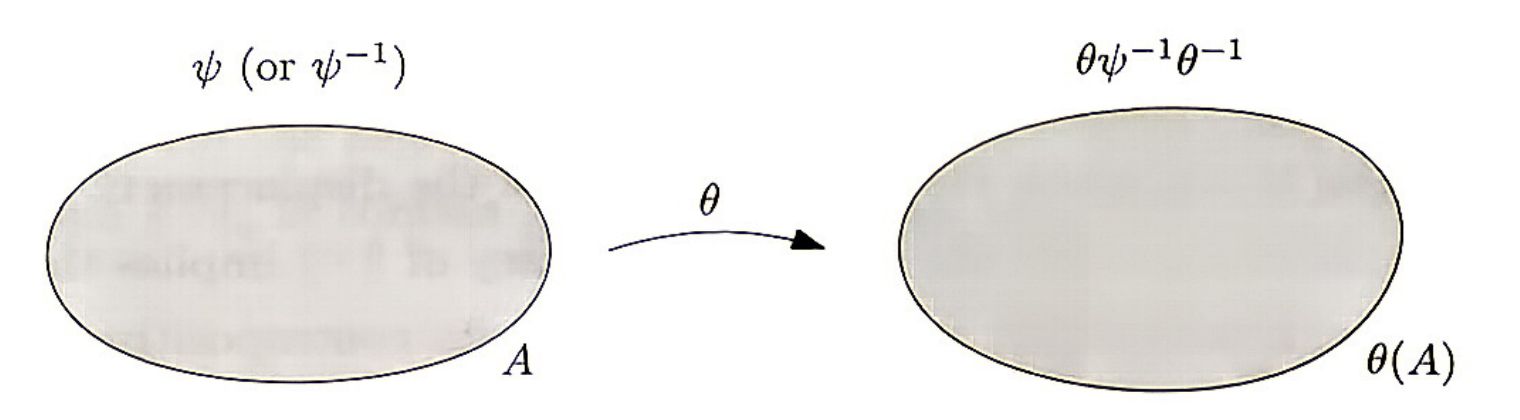
\includegraphics[width=0.72\linewidth]{figures/fig_p153_1.png}
    \caption*{图 6.2\quad $A$ 的位移（原书 p.145, Figure 6.2；PDF p.153）}
  \end{figure}

  于是对二重换位子 $[\varphi,[\psi,\theta]]$，有
  \begin{align*}
    [\varphi,[\psi,\theta]]
    &=\varphi[\psi,\theta]\varphi^{-1}[\psi,\theta]^{-1}\\
    &=\varphi(\psi\theta\psi^{-1}\theta^{-1})\varphi^{-1}
      (\theta\psi\theta^{-1}\psi^{-1})\\
    &=(\varphi\psi\varphi^{-1})(\theta\psi^{-1}\theta^{-1}\theta\psi\theta^{-1})
      \psi^{-1}\\
    &=\varphi\psi\varphi^{-1}\psi^{-1}.
  \end{align*}
  换言之，$[\varphi,\psi]=[\varphi,[\psi,\theta]]$。这里第三个等号来自如下事实：
  $\theta\psi^{-1}\theta^{-1}$ 与 $\varphi^{-1}$ 支撑在不同的区域中（故由练习
  1.7.4，它们可交换）。于是有
  \[
    4\|\theta\|_{\mathrm{Hofer}}\ge 2\|[\psi,\theta]\|_{\mathrm{Hofer}}
    \ge\|[\varphi,[\psi,\theta]]\|_{\mathrm{Hofer}}
    =\|[\varphi,\psi]\|_{\mathrm{Hofer}}>0,
  \]
% >>> p154
  其中第一个不等式来自命题 6.1.2，最后一个不等式来自定理 6.1.1
  （$\|\cdot\|_{\mathrm{Hofer}}$ 的非退化性）。
\end{wproof}

% [Tutor Note: 含糊点拨——定理 6.1.2 的证明隐含了两个不显然的前提：(i) 必须存在
% 支撑在 $A$ 内且不交换的两个哈密顿微分同胚，这用到 $A$ 内部非空（可取一个
% Darboux 球，其上的紧支撑哈密顿微分同胚群非交换）；(ii) 把命题 6.1.2 的换位子
% 估计与定理 6.1.1 的非退化性结合，才能从 $\|[\varphi,\psi]\|_{\mathrm{Hofer}}>0$
% 反推出 $\|\theta\|_{\mathrm{Hofer}}>0$。换言之，$e(A)>0$ 是「硬」的辛现象，
% 其证明同时用到了换位子估计（软）与非退化性（硬）。]

\begin{wrem}{6.1.4}
  注意位移能量 $e(A)$ 在 $\theta\in\Symp(M,\omega)$ 下不变，因为
  \begin{align*}
    e(\theta(A))
    &=\inf\{\|\varphi\|_{\mathrm{Hofer}}\mid
      \varphi\in\Ham(M,\omega),\ \varphi(\theta(A))\cap\theta(A)=\varnothing\}\\
    &=\inf\{\|\varphi\|_{\mathrm{Hofer}}\mid
      \varphi\in\Ham(M,\omega),\ (\theta^{-1}\varphi\theta)(A)\cap A=\varnothing\}
      =e(A),
  \end{align*}
  其中最后一步用到 $\|\cdot\|_{\mathrm{Hofer}}$ 的共轭不变性质。
\end{wrem}

\begin{wexam}{6.1.3}
  [124] 中有一个经典结果：对 $(\R^{2n},\omega_{\mathrm{std}})$ 中的球
  $B^{2n}(r)$，可以算出 $e(B^{2n}(r))=\pi r^2$。后来，[221] 证明：对任意闭
  辛流形，若 $M$ 包含一个半径为 $3r$ 的 Darboux 球 $U$（即，在相差一个辛同胚的
  意义下 $U$ 就是 $B^{2n}(3r)$——见定理 4.3.1），则由注 6.1.4 中的不变性质可推出
  $e(U)=\pi r^2$。\hfill$//$
\end{wexam}

% [Tutor Note: 原文疑误——例 6.1.3 中「$U$ 辛同胚于 $B^{2n}(3r)$」与「$e(U)=\pi r^2$」
% 彼此矛盾：由同一例前半部分与注 6.1.4 的不变性，应有
% $e(U)=e(B^{2n}(3r))=\pi(3r)^2=9\pi r^2$。合理的读法是：$M$ 中含半径 $3r$ 的
% Darboux 球时，其中半径 $r$ 的球（而非整个 $U$）满足 $e=\pi r^2$；作者可能把
% 「半径为 $r$ 的球」误写成了 $U$。已记入 review_ch06.md，待人工核对原文。]

\begin{wrem}{6.1.5}
  M.~Usher 在 [226] 的推论 1.6 中证明了一个相当出人意料的结果：$e(A)$ 的计算
  可以大大简化，即
  \[
    e(A)=\inf_{\varphi_H^1(A)\cap A=\varnothing}
    \int_0^1\left(\max_A H_t-\min_A H_t\right)dt.
  \]
  注意：积分中的 Hofer 范数是在 $A$ 上取的（而非原始定义 (6.1) 中的整个流形 $M$）。
\end{wrem}

% [Tutor Note: 易错预警——注 6.1.5 的公式与 (6.1) 的区别仅在 $\max$、$\min$ 的取法：
% 由「$M$ 上」改为「$A$ 上」。正是这一改动把 $e(A)$ 变成了只依赖 $A$（及其辛邻域）
% 的量，从而可以用于定义辛容量。抄录时务必不要漏掉下标 $A$；同时注意下确界是对
% 满足 $\varphi_H^1(A)\cap A=\varnothing$ 的时间 1 映射取的，$H$ 未必规范化。]

可以把 $e(A)$ 定义中的 $\|\cdot\|_{\mathrm{Hofer}}$ 换成 $\Ham(M,\omega)$ 上任意
其他的双不变伪度量 $\|\cdot\|$，从而得到位移能量的一种变体，记作
$e_{\|\cdot\|}$。此时同样的论证表明：$\|\cdot\|$ 的非退化性蕴含对任意内部非空的
子集 $A$ 有 $e_{\|\cdot\|}(A)>0$。有时其逆否命题更为有用：在闭辛流形
$(M,\omega)$ 上，若存在内部非空的子集 $A\subset M$ 使得 $e_{\|\cdot\|}(A)=0$，则
伪度量 $\|\cdot\|$ \emph{不}非退化，且恒等于零。

% [Tutor Note: 术语/记号依据——「双不变伪度量」对应 bi-invariant pseudo-metric，
% 即同时保持左、右乘的伪度量；「共轭不变伪范数」对应 conjugate invariant
% pseudo-norm。二者在 $\Ham$ 中通过 $d(\varphi,\psi)=\|\varphi^{-1}\psi\|$ 一一对应。
% 这句话是本节的「反向使用」：位移能量为零可以作为伪度量退化的判别准则，第 7 章
% 的形不变量（shape invariant）正是沿此思路展开的。]

\begin{wexer}{6.1.4}
  设群 $G$ 上配有共轭不变范数 $\|\cdot\|$。考虑一个在 $G$ 上传递地作用的集合 $S$。
  该共轭不变范数在 $S$ 上诱导一个伪度量 $\delta_{\|\cdot\|}$，定义为
  \[
    \delta_{\|\cdot\|}(s_1,s_2)=\inf\{\|g\|\mid gs_1=s_2\},
  \]
  其中 $s_1,s_2\in S$。现在固定基点 $s_0\in S$，并令
  $H=\{g\in G\mid gs_0=s_0\}$。证明：$H$ 关于 $\|\cdot\|$ 在 $G$ 上诱导的拓扑的
  闭包是一个子群，且由
  \[
    \bar{H}=\{g\in G\mid \delta_{\|\cdot\|}(s_0,gs_0)=0\}
  \]
  给出。特别地，$\delta_{\|\cdot\|}$ 非退化当且仅当 $H$ 是闭的。
\end{wexer}

% [Tutor Note: 含糊点拨——练习 6.1.4 是「齐性空间上由范数诱导度量」的标准构造，
% 其要点是：$\delta_{\|\cdot\|}$ 非退化意味着稳定子 $H$ 闭，即 $S\cong G/H$ 是
% $T_1$ 空间；证明中用三角不等式与共轭不变性说明 $\bar H$ 对乘法封闭。该练习是
% 第 7 章把 Hofer 几何搬到拉格朗日 Grassmann 流形上的技术准备。]

% >>> p155
为结束本节，我们简要提及切触几何中一个类似的故事。给定切触流形
$(M,\xi)$ 与群 $\mathrm{Cont}_0(M,\xi)$，人们或许会问：$\mathrm{Cont}_0(M,\xi)$ 上
是否存在 Hofer 型的共轭不变范数？在 [203] 中，Shelukhin 在固定一个切触
1-形式之后，于 $\mathrm{Cont}_0(M,\xi)$ 上构造了一个 Hofer 型范数。具体地说，对
任意 $\varphi\in\mathrm{Cont}_0(M,\xi)$ 以及满足 $\xi=\ker\alpha$ 的切触 1-形式
$\alpha$，任意连接 $\mathbf{1}$ 与 $\varphi$ 的切触同痕
$\{\varphi_t\}_{t\in[0,1]}$ 都唯一确定一个哈密顿函数
$h\colon[0,1]\times M\to\R$（见命题 3.5.1）。于是考虑
\[
  \|\varphi\|_\alpha:=\inf\left\{
  \int_0^1\max_M|h_t|\,dt\;\middle|\;
  \begin{array}{l}
    h\ \text{生成一条连接}\ \mathbf{1}\ \text{与映射}\ \varphi\ \text{的}\\
    \text{切触同痕}
  \end{array}\right\}.
\]
遗憾的是，$\|\cdot\|_\alpha$ \emph{不}是共轭不变的。事实上，[196] 中的命题
1.5（它受 [36] 中定理 1.11 (i) 的启发）给出了一个漂亮的结果：任何非平凡的
共轭不变范数在 $\mathrm{Cont}_0(M,\xi)$ 上都必须是离散的（特别地，它不能任意小！）。
确实，假设存在一个可以逼近 $0$ 的共轭不变范数 $\|\cdot\|$。取定一个 Darboux 球
$B\subset M$，以及 $\varphi,\psi\in\mathrm{Cont}_0(M,\xi)$，它们支撑在 $B$ 中且
$[\varphi,\psi]\ne\mathbf{1}$。于是可以找到 $\theta\in\mathrm{Cont}_0(M,\xi)$，
使得 $\theta(B)\subset B(\varepsilon)$（一个非常小的球），且
$\theta\varphi\theta^{-1}$、$\theta\psi\theta^{-1}$ 均支撑在 $B(\varepsilon)$ 中。
注意存在 $\tau\in\mathrm{Cont}_0(M,\xi)$ 能位移 $B(\varepsilon)$，且
$\|\tau\|\le\varepsilon$。于是
\[
  \|[\theta\varphi\theta^{-1},\theta\psi\theta^{-1}]\|
  =\|\theta[\varphi,\psi]\theta^{-1}\|=\|[\varphi,\psi]\|>0,
\]
但 $\|[\theta\varphi\theta^{-1},\theta\psi\theta^{-1}]\|\le 4\|\tau\|$，而
$\|\tau\|$ 可任意小。于是得到矛盾。尽管缺少共轭不变性质，$\|\cdot\|_\alpha$ 在
切触几何中仍有大量应用（见 [203,187,227]）。
